\documentclass[11pt,twoside,a4paper]{article}
\usepackage{amsmath}
\usepackage{graphicx}

\begin{document}

	\begin{figure}
		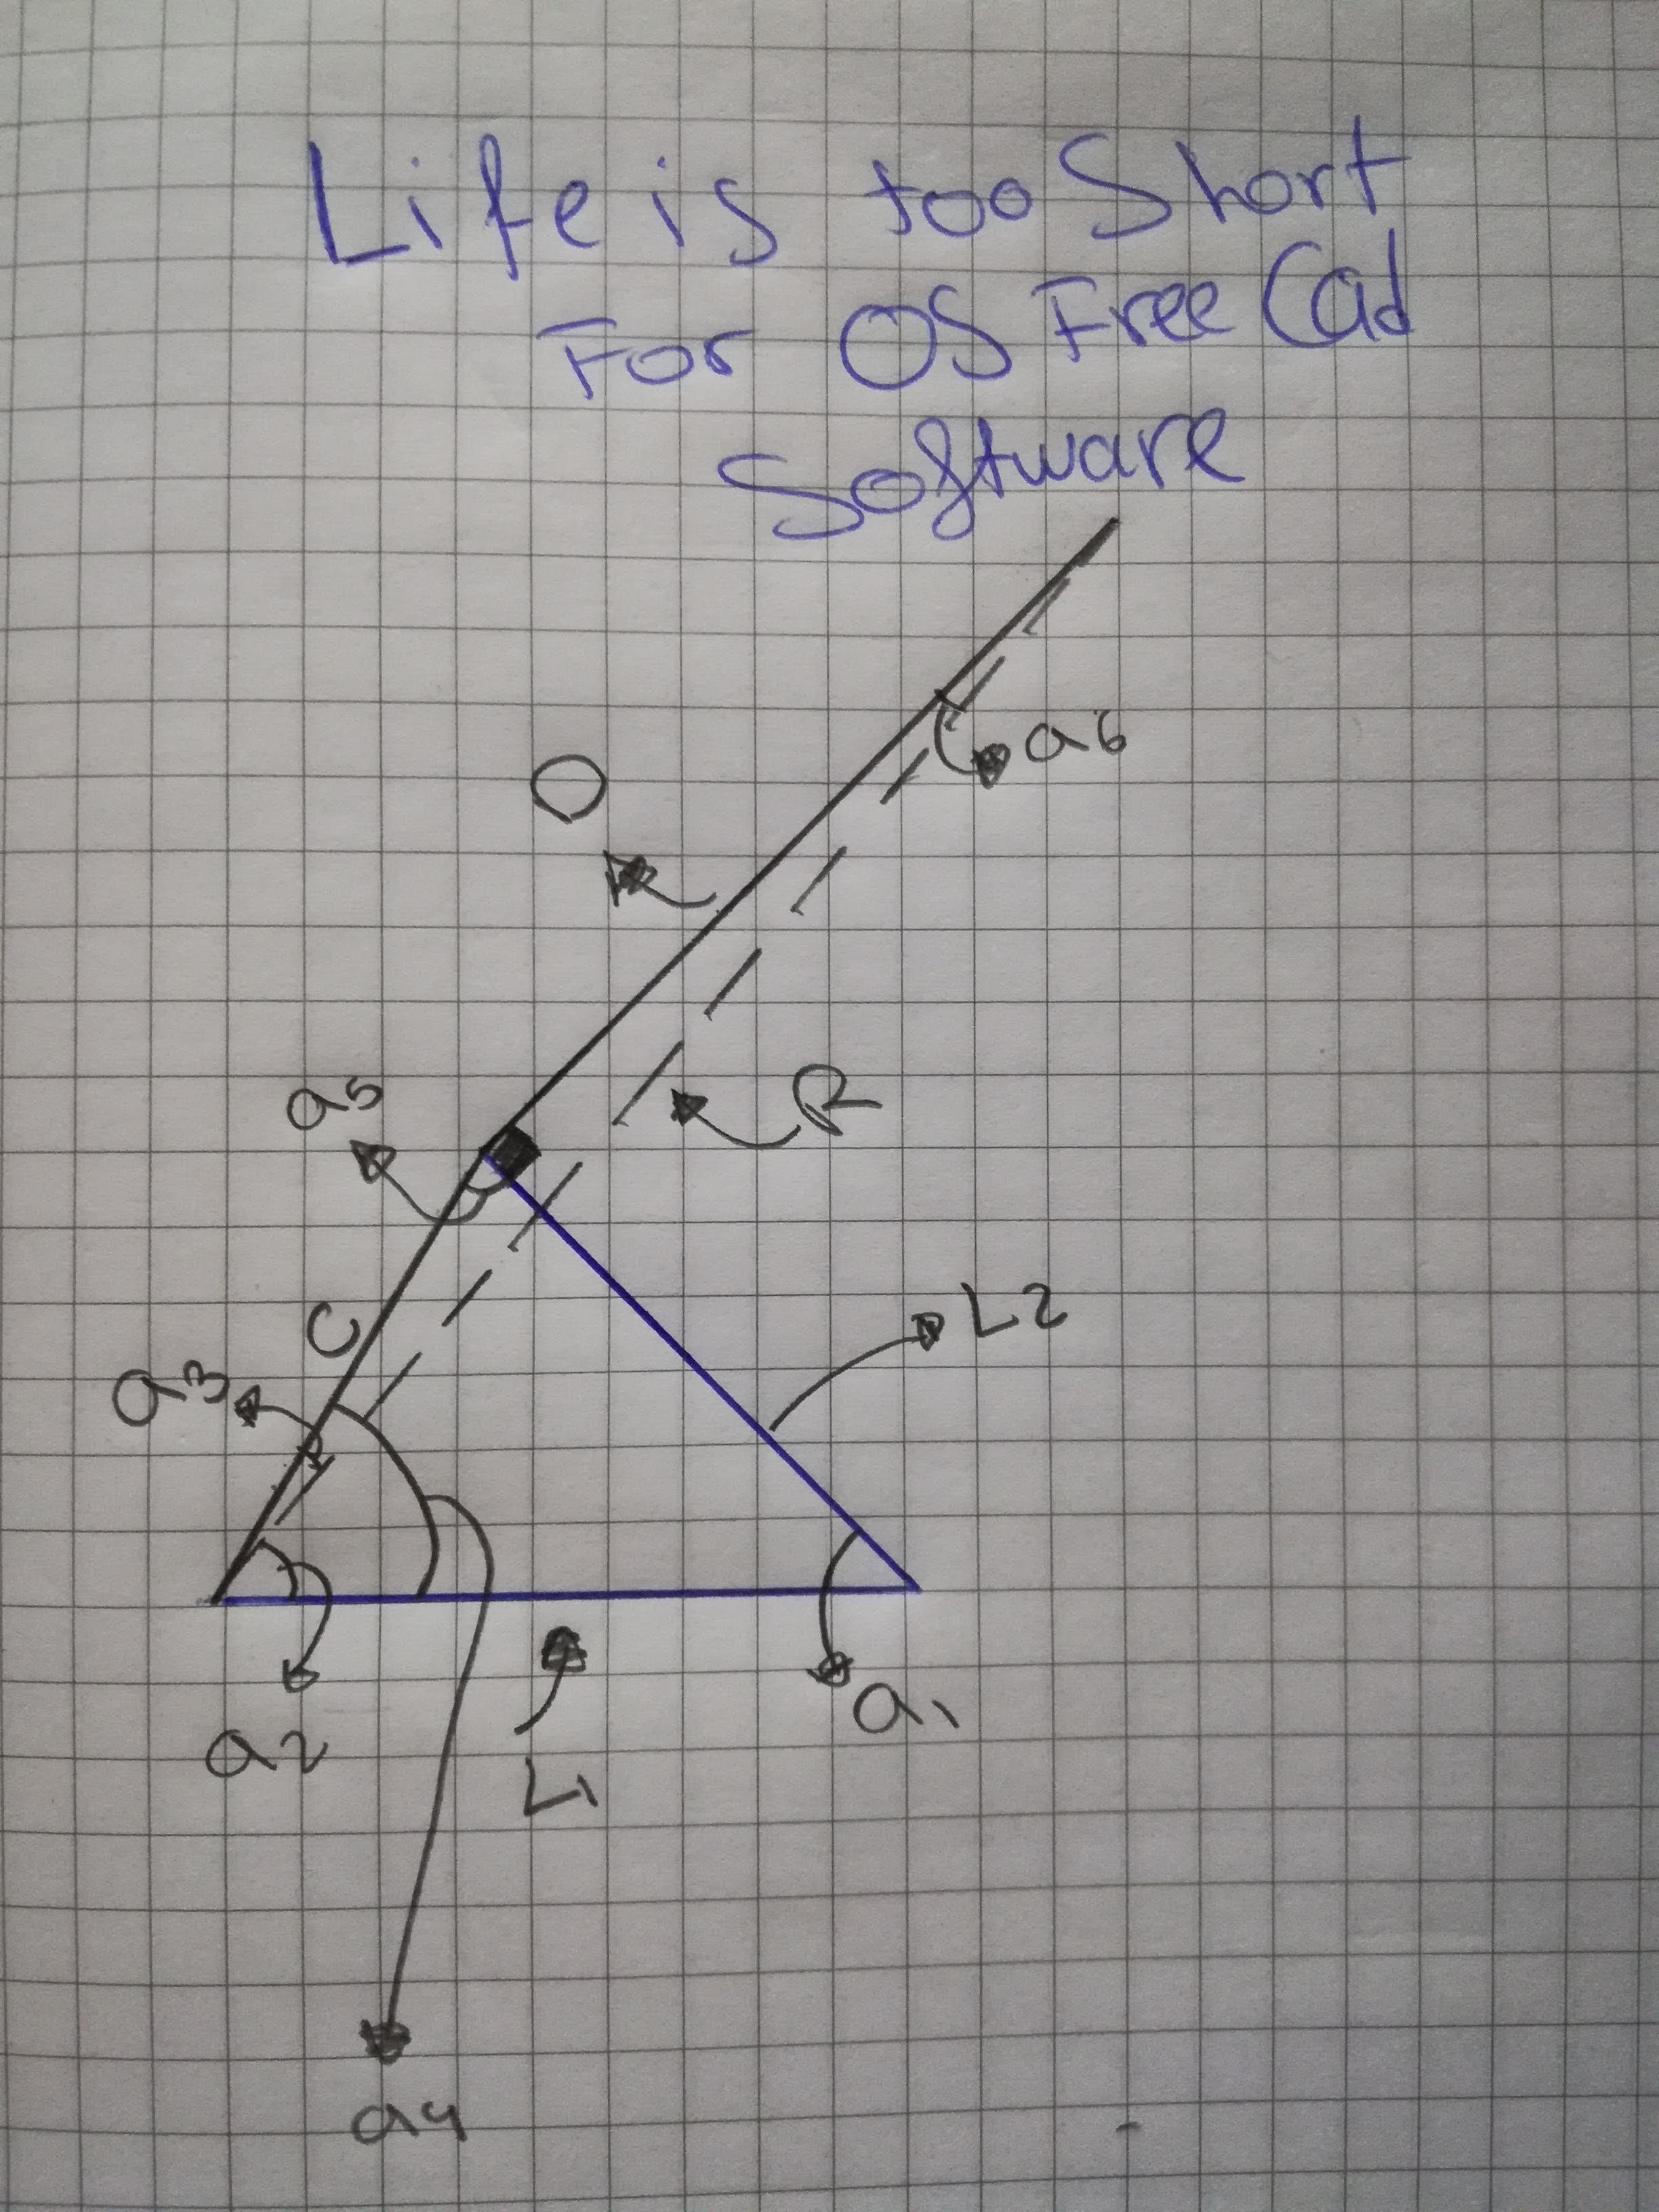
\includegraphics[scale=0.2,natwidth=2448,natheight=3264]{../docs/equation.jpg}
	\end{figure}

	By applying the cosin rule on the $L_1$ $L_2$ C triangle:

	\begin{equation}
		C^2 = L_1^2 + L_2^2 -2 L_1 L_2 \cos a_1
	\end{equation}

	By applying the sine rule on the $L_1$ $L_2$ C triangle:
	
	\begin{align*}
		\frac{L_1}{\sin a_5} &= \frac{C}{\sin a_1}\\
		a_5 &= \arcsin \left(\frac{L_1 . \sin a_1}{C}\right)
	\end{align*}
	
	By Combining (1) and (2):
	
	\begin{equation}
		a_5 = \arcsin \left(\frac{L_1 . \sin a_1}{\sqrt{L_1^2 + L_2^2 - 2 L_1.L_2.\cos a_1}}\right)
	\end{equation}
	
	By applying the cosin rule on the R C D triangle:
	
	\begin{equation}
		R^2 = C^2 + D^2 - 2.C.D\cos(a_5+90)
	\end{equation}
	
	By applying the sine rule on the R C D triangle:
	
	\begin{equation}
		\frac{•}{•}
	\end{equation}

\end{document}